\section*{Binary batch size effect on run
speed}

2018/07/26 - SYNALP - Esteban MARQUER

\subsection{Context}

It has been said that batches using binary sizes (64, 256, 1024,
\ldots{}) perform faster than non-binary sises.

\subsection{Paradigm}

To verify this phenomenon and perhaps improve the training speed, a
comparative experiment has been done with a batch size of 128 and a
batch size of 200.

\subsection{Results}

There is notable no effect, except the effect predicted by the batch
size comparision done previously, and stating that batches with a size
of 200 are faster than with a size of 128.

\begin{figure}[ht]
\centering
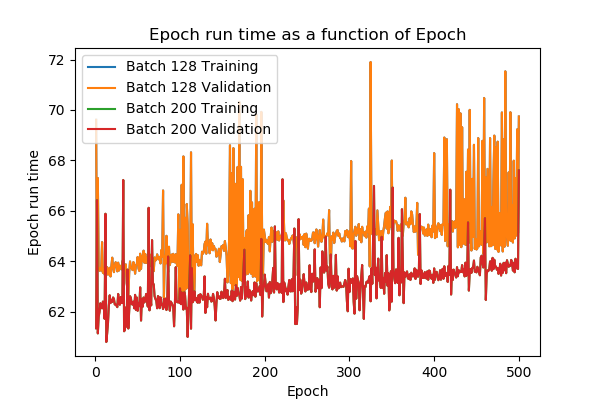
\includegraphics{parts/appendix/reports-papud/2018_07_26-Binary_batch_size/time_epoch.png}
\caption{time per epoch}
\end{figure}

\subsection{Conclusion}

The most straightforward conclusion is that either the effect of binary
sizes is negligible if not non-existent, or there is a hidden parameter
changing th true size of the data (for example a set of bytes used to
store metadata together with the regular data).

As the previous batch size (200) performs better, we will keep it.

\subsection{Next steps and
improvements}

Investigating a potentially non-existent effect (at least with the
current model) does not seem efficient considering the potential gain in
computation time (compared to improving the naive model).

No further work will be done on that now (at least for now).
